\chapter{Catálisis organometálica: etapas elementales y ciclos}\label{ch:b2:catalytic-cycles}

Unos miligramos de una sal de paladio pueden unir dos anillos \omterm{def:b2:huckel:aromatic}{aromáticos} en un matraz
que contiene kilogramos de reactivos: el mismo átomo metálico hace el trabajo miles de
veces, volviendo a su estado inicial tras cada paso. Cómo lo hace lo
cuenta un \omterm{def:b2:catalytic-cycles:cycle}{ciclo catalítico}, una secuencia cerrada de un puñado de etapas elementales.
Solo hay unos pocos tipos de etapas, y cada uno cambia el estado de oxidación, el
recuento de electrones y el número de ligandos del metal de un modo fijo. Con el
recuento de electrones del \cref{ch:b2:coordination-complexes}, un ciclo puede leerse,
comprobarse y, a veces, predecirse.

\begin{recall}
\Cref{ch:b2:coordination-complexes}: estado de oxidación, $d^n$, \omterm{def:b2:coordination-complexes:electron-count}{recuento de electrones de valencia},
\omterm{def:b2:coordination-complexes:electron-count}{regla de los 18 electrones}, \omterm{def:b2:coordination-complexes:hapticity}{hapticidad}. \Cref{ch:b2:ligand-field}: ligandos $\pi$-aceptores y
\omterm{def:b2:ligand-field:pi-ligands}{retrodonación}. El volumen del primer año: catalizador, catálisis homogénea, etapa elemental,
etapa determinante de la velocidad, compuesto organometálico, número de oxidación.
\end{recall}

\begin{omfigure}
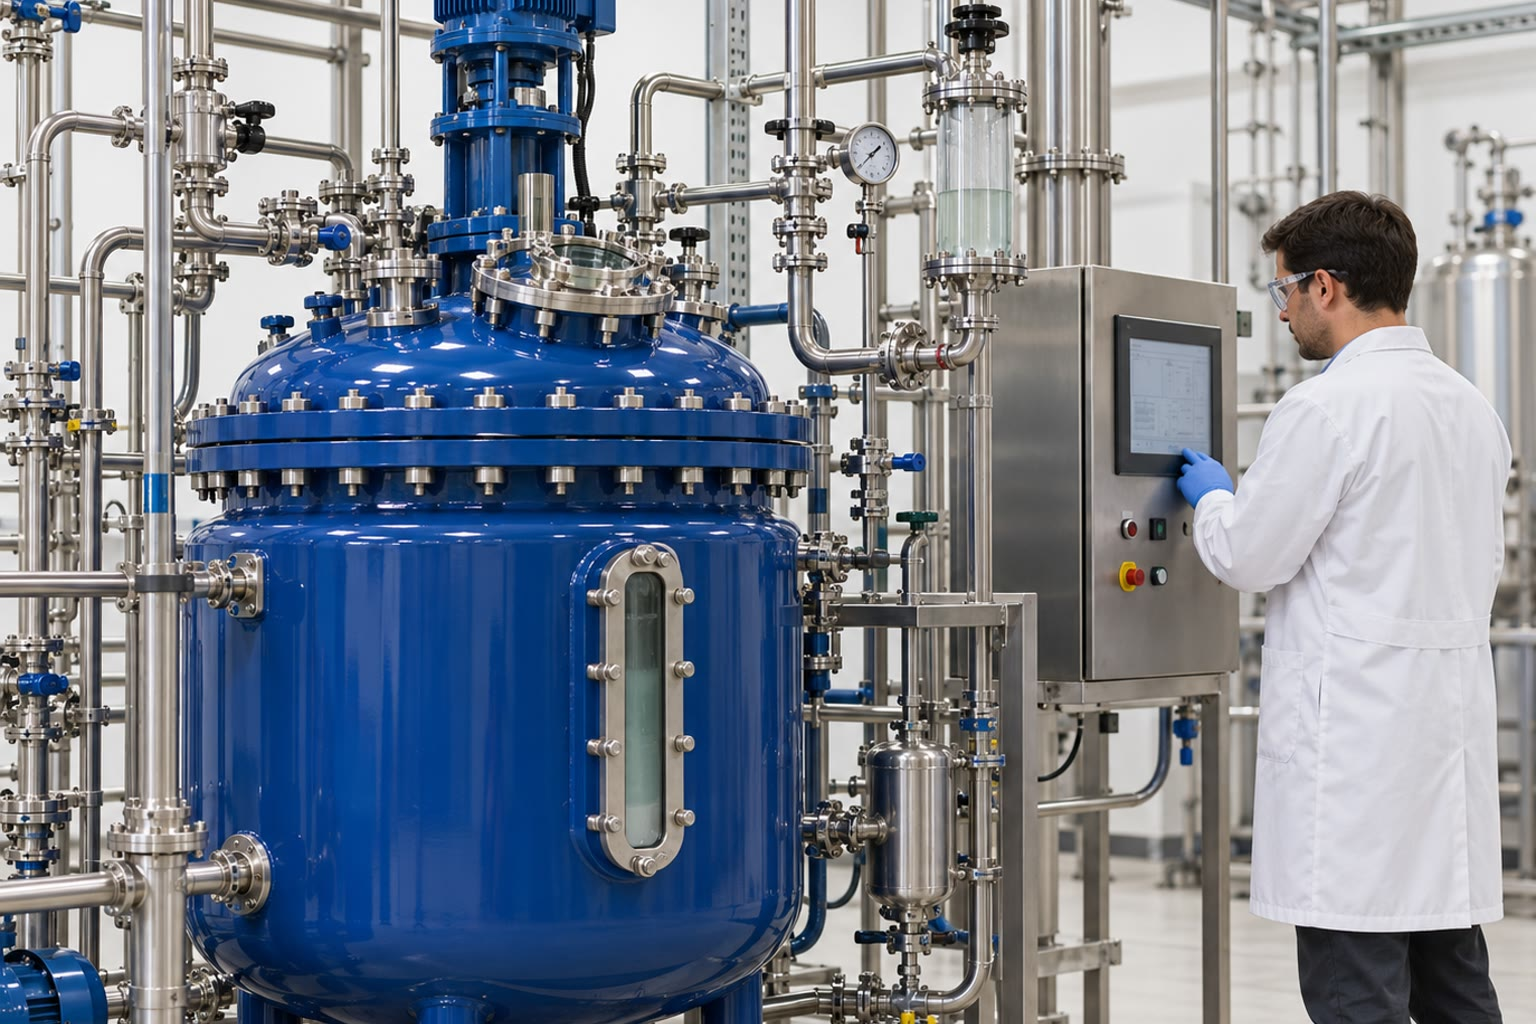
\includegraphics[width=0.62\linewidth]{images/book3/ai/b2-20-pilot-plant.jpg}

{\small Una planta piloto de química de procesos: un reactor de acero vitrificado, donde un
acoplamiento catalizado se escala a partir del matraz antes de la producción.}
\end{omfigure}

\section{El lenguaje de los complejos organometálicos}

Los complejos organometálicos se cuentan como en el \cref{met:b2:coordination-complexes:electron-count},
con algunos ligandos más: un hidruro \ce{H-} y un anión alquilo o arilo \ce{R-} aportan dos
electrones cada uno y cuentan $-1$ en el estado de oxidación; \ce{CO}, las fosfinas \ce{PR3} y
los $\eta^2$-alquenos aportan dos electrones y cuentan 0; un haluro \ce{X-} aporta dos y cuenta
$-1$.

\begin{definition}[Complejos insaturados]\label{def:b2:catalytic-cycles:unsaturated}
Un \emph{complejo coordinativamente insaturado}\index{complejo coordinativamente insaturado}
tiene menos de 18 electrones de valencia (a menudo 16) y puede unirse a otro ligando: tiene una
\emph{posición vacante}\index{posicion vacante@posición vacante}, una posición de su \omterm{def:b2:coordination-complexes:coordination-sphere}{esfera de coordinación} libre para
recibir a un dador de dos electrones.
\end{definition}

Los complejos $d^8$ plano-cuadrados del rodio(I), el iridio(I), el paladio(II) y el
platino(II) son complejos de 16 electrones; las bisfosfinas de paladio(0) \ce{PdL2} tienen 14.
Estos complejos son las especies activas de la mayoría de los \omterm{def:b2:catalytic-cycles:cycle}{ciclos catalíticos}.

\begin{method}[Contar un complejo organometálico]\label{met:b2:catalytic-cycles:count-organometallic}
\begin{enumerate}
  \item Enumérense los ligandos: aniónicos (\ce{H-}, \ce{R-}, \ce{X-}, \ce{C5H5-}) y neutros
        (\ce{CO}, \ce{PR3}, alquenos, disolvente).
  \item Estado de oxidación = carga del complejo $-$ suma de las cargas de los ligandos aniónicos.
  \item $n = g -$ estado de oxidación; recuento = $n + 2 \times$(número de dadores de dos electrones)
        $+$ 6 por $\eta^5$-\ce{C5H5-}.
  \item Número de coordinación = número de posiciones de ligando ocupadas.
\end{enumerate}
\end{method}

\section{Intercambio de ligandos, adición oxidante, eliminación reductora}

\begin{definition}[Intercambio de ligandos]\label{def:b2:catalytic-cycles:ligand-exchange}
Un \emph{intercambio de ligandos}\index{intercambio de ligandos} es una etapa elemental en la que un ligando de
la \omterm{def:b2:coordination-complexes:coordination-sphere}{esfera de coordinación} es sustituido por otro; no cambia ni el estado de oxidación
ni, en conjunto, el recuento de electrones. Sus mecanismos se estudian en el volumen del tercer año.
\end{definition}

\begin{definition}[Adición oxidante y eliminación reductora]\label{def:b2:catalytic-cycles:oxidative-addition}
En una \emph{adición oxidante}\index{adicion oxidante@adición oxidante}, una molécula A--B se adiciona a un
centro metálico rompiendo su enlace A--B y formando los enlaces M--A y M--B. Una
\emph{eliminación reductora}\index{eliminacion reductora@eliminación reductora} es la etapa inversa: dos
ligandos A y B, en cis entre sí, se unen en A--B y abandonan el metal.
\end{definition}

\begin{proposition}[Recuento de una adición oxidante]\label{prop:b2:catalytic-cycles:oa}
Una \omterm{def:b2:catalytic-cycles:oxidative-addition}{adición oxidante} eleva en 2 el estado de oxidación del metal, su \omterm{def:b2:coordination-complexes:electron-count}{recuento de electrones de valencia}
en 2 y su número de coordinación en 2; una \omterm{def:b2:catalytic-cycles:oxidative-addition}{eliminación reductora} rebaja cada uno en 2.
\end{proposition}

\begin{proof}
A y B se cuentan como aniones (\ce{H-}, \ce{R-}, \ce{X-}) una vez unidos: dos nuevos ligandos
aniónicos elevan en 2 el estado de oxidación y rebajan $n$ en 2; aportan dos pares, $+4$
electrones; el recuento cambia en $-2 + 4 = +2$. Se ocupan dos posiciones nuevas. La
etapa inversa invierte cada cambio.
\end{proof}

\begin{example}[El complejo de Vaska]\label{ex:b2:catalytic-cycles:vaska}
\ce{[IrCl(CO)(PPh3)2]}, plano-cuadrado: iridio(I), $d^8$, 16 electrones, tetracoordinado.
Adiciona dihidrógeno: \ce{[IrH2Cl(CO)(PPh3)2]}, iridio(III), $d^6$, 18 electrones, octaédrico,
con los dos hidruros en cis.
\end{example}

\section{Inserción, eliminación, transmetalación}

\begin{definition}[Inserción y eliminación de $\beta$-hidruro]\label{def:b2:catalytic-cycles:insertion}
En una \emph{inserción migratoria}\index{insercion migratoria@inserción migratoria}, un ligando insaturado
(alqueno, \ce{CO}) unido al metal se inserta en un enlace M--H o M--C en cis: \ce{M-H} y un
alqueno dan un alquilo \ce{M-CH2-CH2-H}; \ce{M-R} y \ce{CO} dan un acilo \ce{M-C(=O)R}.
Una \emph{eliminación de $\beta$-hidruro}\index{eliminacion de beta-hidruro@eliminación de $\beta$-hidruro}
es la inversa de una inserción de alqueno: un hidrógeno del carbono en $\beta$ respecto del
metal pasa al metal, y se libera un alqueno.
\end{definition}

\begin{proposition}[Recuento de una inserción]\label{prop:b2:catalytic-cycles:insertion}
Una \omterm{def:b2:catalytic-cycles:insertion}{inserción migratoria} conserva el estado de oxidación y rebaja el recuento de electrones en 2
(se libera una posición de ligando); una eliminación de $\beta$-hidruro eleva el recuento en 2.
\end{proposition}

\begin{proof}
Antes: \ce{H-} (o \ce{R-}, aniónico) y el alqueno (neutro), dos ligandos, cuatro electrones.
Después: un alquilo (aniónico), dos electrones. La carga aniónica no cambia: mismo
estado de oxidación; se pierden dos electrones y una posición.
\end{proof}

\begin{proposition}[Condiciones de la eliminación de $\beta$-hidruro]\label{prop:b2:catalytic-cycles:beta-h}
Un alquilo metálico solo sufre eliminación de $\beta$-hidruro si el alquilo lleva un hidrógeno en
su carbono $\beta$ y el metal tiene una \omterm{def:b2:catalytic-cycles:unsaturated}{posición vacante} en cis respecto del alquilo.
\end{proposition}

\begin{proof}[Argumento]
La etapa transcurre a través de una disposición de cuatro eslabones M--C$_\alpha$--C$_\beta$--H en la que el
hidrógeno alcanza el metal: necesita ese hidrógeno, y una posición vacía junto al alquilo
para recibirlo. Los grupos metilo, bencilo, neopentilo y arilo, que no tienen ningún hidrógeno en $\beta$
capaz de alcanzar el metal, son estables frente a ella.
\end{proof}

\begin{definition}[Transmetalación]\label{def:b2:catalytic-cycles:transmetalation}
Una \emph{transmetalación}\index{transmetalacion@transmetalación} transfiere un grupo orgánico de un metal
(o metaloide: boro, cinc, estaño) a otro, normalmente a cambio de un haluro.
\end{definition}

\begin{omfigure}
\begin{tikzpicture}[font=\small, >={Stealth}]
  \tikzset{omstepar/.style={->, thick}}
  \foreach \y/\l/\r/\top/\bot/\rev in {
      0/{$\mathrm{L}_n\mathrm{M}$}/{$\mathrm{L}_n\mathrm{M(A)(B)}$}/{+ A--B}/{adición oxidante}/{eliminación reductora},
      -1.5/{$\mathrm{L}_n\mathrm{M(H)(CH_2{=}CH_2)}$}/{$\mathrm{L}_n\mathrm{M{-}CH_2CH_3}$}/{}/{inserción migratoria}/{eliminación de $\beta$-hidruro},
      -3.0/{$\mathrm{L}_n\mathrm{M(X)(R)}$}/{$\mathrm{L}_n\mathrm{M(R)(R')}$}/{+ R$'$--[B], $-$ X--[B]}/{transmetalación}/{},
      -4.5/{$\mathrm{L}_n\mathrm{M(X)}$}/{$\mathrm{L}_n\mathrm{M(X)(L')}$}/{+ L$'$}/{intercambio o unión de ligando}/{}} {
    \node[cyclenode, anchor=east] (l) at (0,\y) {\l};
    \node[cyclenode, anchor=west] (r) at (5.2,\y) {\r};
    \draw[omstepar] ($(l.east)+(0.1,0.08)$) -- ($(r.west)+(-0.1,0.08)$) node[midway, above, font=\scriptsize] {\top};
    \node[font=\scriptsize, anchor=north] at (2.6,\y-0.02) {\bot};
    \node[font=\scriptsize, black!55, anchor=west] at (5.2,\y-0.5) {\rev};
  }
\end{tikzpicture}

{\small Las etapas elementales de la catálisis organometálica. \omterm{def:b2:catalytic-cycles:oxidative-addition}{Adición oxidante}: estado de
oxidación, recuento y número de coordinación $+2$; \omterm{def:b2:catalytic-cycles:oxidative-addition}{eliminación reductora}: $-2$. \omterm{def:b2:catalytic-cycles:insertion}{Inserción
migratoria}: recuento $-2$, estado de oxidación sin cambios; eliminación de $\beta$-hidruro: la
inversa. \omterm{def:b2:catalytic-cycles:transmetalation}{Transmetalación}: un grupo orgánico pasa al metal desde el boro, el cinc o el estaño.}
\end{omfigure}

\section{Lectura de un ciclo catalítico}

\begin{definition}[Ciclo catalítico]\label{def:b2:catalytic-cycles:cycle}
Un \emph{ciclo catalítico}\index{ciclo catalitico@ciclo catalítico} es una secuencia cerrada de etapas elementales
que consume los reactivos, libera los productos y regenera su primer complejo. El
compuesto añadido a la reacción, que se convierte en el primer complejo del ciclo, es el
\emph{precatalizador}\index{precatalizador}. El \emph{número de recambio}\index{numero de recambio@número de recambio}
(TON) es la cantidad de producto formada por cantidad de catalizador; la \emph{frecuencia de
recambio}\index{frecuencia de recambio} (TOF) es el número de recambio por unidad de tiempo.
\end{definition}

\begin{proposition}[La ecuación global]\label{prop:b2:catalytic-cycles:cycle-sum}
La suma de las etapas de un \omterm{def:b2:catalytic-cycles:cycle}{ciclo catalítico} es la ecuación de la reacción catalizada:
cada complejo metálico aparece una vez como producto y otra como reactivo, y se cancela.
\end{proposition}

\begin{proof}
Al ser cerrado el ciclo, cada intermedio se forma en una etapa y se consume en la siguiente;
al sumar las etapas, estas especies aparecen en ambos miembros y se cancelan. Lo que queda son las
especies que entran desde fuera (reactivos) y las que salen (productos).
\end{proof}

\begin{method}[Leer un ciclo]\label{met:b2:catalytic-cycles:read-cycle}
\begin{enumerate}
  \item Para cada complejo, calcúlense el estado de oxidación, el recuento de electrones y el
        número de coordinación.
  \item Nómbrese cada etapa a partir de los cambios ($+2/+2/+2$: \omterm{def:b2:catalytic-cycles:oxidative-addition}{adición oxidante}; recuento $-2$ a
        estado de oxidación constante: inserción; y así sucesivamente).
  \item Compruébese que ningún complejo supera los 18 electrones y que una etapa que necesita una \omterm{def:b2:catalytic-cycles:unsaturated}{posición vacante}
        parte de un complejo insaturado.
  \item Súmense las etapas: la suma debe ser la ecuación global.
\end{enumerate}
\end{method}

\begin{omfigure}
\begin{tikzpicture}[font=\small, >={Stealth}]
  \node[cyclenode] (n1) at (90:2.3) {\ce{[RhCl(PPh3)2]}\\ Rh(I), 14 e};
  \node[cyclenode] (n2) at (0:3.4) {\ce{[RhH2Cl(PPh3)2]}\\ Rh(III), 16 e};
  \node[cyclenode] (n3) at (270:2.3) {\ce{[RhH2Cl(PPh3)2(RCH=CH2)]}\\ Rh(III), 18 e};
  \node[cyclenode] (n4) at (180:3.4) {\ce{[RhH(CH2CH2R)Cl(PPh3)2]}\\ Rh(III), 16 e};
  \draw[cyclearc] (n1) to[bend left=20] node[cyclelabel, below left] {adición\\ oxidante} (n2);
  \draw[cyclearc] (n2) to[bend left=20] node[cyclelabel, left=12pt] {unión del\\ alqueno} (n3);
  \draw[cyclearc] (n3) to[bend left=20] node[cyclelabel, above right] {inserción\\ migratoria} (n4);
  \draw[cyclearc] (n4) to[bend left=20] node[cyclelabel, below right] {eliminación\\ reductora} (n1);
  \draw[cyclein] (4.6,2.3) node[right] {\ce{H2}} -- (2.6,1.75);
  \draw[cyclein] (4.6,-2.3) node[right] {alqueno} -- (2.6,-1.75);
  \draw[cycleout] (-2.6,1.75) -- (-4.6,2.3) node[left] {alcano};
  \node[font=\scriptsize, align=center, black!60] at (0,-0.05) {precatalizador\\ \ce{[RhCl(PPh3)3]}\\ pierde una \ce{PPh3}};
\end{tikzpicture}

{\small La hidrogenación de un alqueno con el catalizador de Wilkinson, simplificada (se omiten los intercambios de fosfina
y de disolvente). Las cuatro etapas suman $\ce{RCH=CH2 + H2 -> RCH2CH3}$; los
complejos de rodio se cancelan.}
\end{omfigure}

\begin{omfigure}
\begin{tikzpicture}[font=\small, >={Stealth}]
  \node[cyclenode] (s1) at (90:2.3) {\ce{PdL2}\\ Pd(0), 14 e};
  \node[cyclenode] (s2) at (0:3.4) {\ce{[ArPd(Br)L2]}\\ Pd(II), 16 e};
  \node[cyclenode] (s3) at (270:2.3) {$[\mathrm{ArPd(Ar')L_2}]$\\ Pd(II), 16 e};
  \draw[cyclearc] (s1) to[bend left=25] node[cyclelabel, below left] {adición\\ oxidante} (s2);
  \draw[cyclearc] (s2) to[bend left=25] node[cyclelabel, above left] {transmetalación} (s3);
  \draw[cyclearc] (s3) to[bend left=35] node[cyclelabel, right] {eliminación\\ reductora} (s1);
  \draw[cyclein] (4.8,2.2) node[right] {\ce{Ar-Br}} -- (2.6,1.6);
  \draw[cyclein] (5.4,-0.9) node[right, align=left] {$\mathrm{Ar'B(OH)_2}$\\ + base} -- (3.3,-1.2);
  \draw[cycleout] (2.3,-2.0) -- (4.4,-2.9) node[right] {\ce{Br-}, \ce{B(OH)3}};
  \draw[cycleout] (-1.75,-0.4) -- (-4.2,-0.4) node[left] {$\mathrm{Ar{-}Ar'}$};
\end{tikzpicture}

{\small El acoplamiento de Suzuki, simplificado. El paladio(0) adiciona el bromuro de arilo; la base
convierte el ácido borónico en un borato, que transfiere su grupo arilo al paladio; los dos
arilos, en cis, se eliminan como el biarilo, y se regenera el paladio(0).}
\end{omfigure}

En la reacción de Heck, el complejo aril--paladio formado por \omterm{def:b2:catalytic-cycles:oxidative-addition}{adición oxidante} une un
alqueno en lugar de un borato; la \omterm{def:b2:catalytic-cycles:insertion}{inserción migratoria} pone el arilo sobre el alqueno, y una
eliminación de $\beta$-hidruro libera el alqueno sustituido (normalmente el isómero trans)
y un hidruro de paladio, del que una base elimina \ce{HBr} para regenerar el paladio(0).

La hidroformilación, la adición de \ce{H2} y \ce{CO} a un alqueno para dar un aldehído,
transcurre con hidruros de cobalto o de rodio mediante la inserción del alqueno, la inserción de \ce{CO}
en el enlace metal--alquilo, la \omterm{def:b2:catalytic-cycles:oxidative-addition}{adición oxidante} de \ce{H2} y la \omterm{def:b2:catalytic-cycles:oxidative-addition}{eliminación reductora} del
aldehído. El sentido de la primera inserción decide el producto: el metal sobre el
carbono terminal da el aldehído lineal, y sobre el carbono interno, el ramificado; las fosfinas
voluminosas favorecen el producto lineal.

\begin{history}[Acoplamientos cruzados]
\begin{minipage}[t]{0.36\linewidth}
\vspace{0pt}
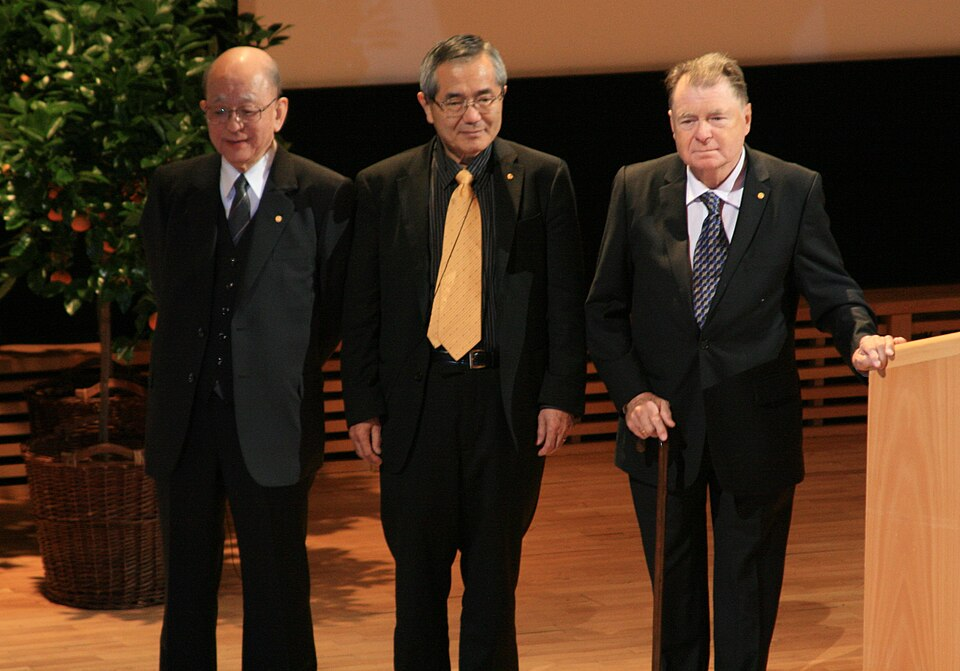
\includegraphics[width=\linewidth]{images/book3/nobel-2010.jpg}
\end{minipage}\hfill
\begin{minipage}[t]{0.6\linewidth}
\vspace{0pt}
Los acoplamientos catalizados por paladio de haluros de arilo y de vinilo con alquenos (Richard Heck, desde
1968), con reactivos organocíncicos (Ei-ichi Negishi, 1977) y con compuestos organobóricos
(Akira Suzuki, 1979) convirtieron en rutina la unión de dos esqueletos carbonados; hoy figuran entre
las reacciones más usadas en la fabricación de medicamentos y materiales. El Premio Nobel de
Química se concedió a los tres en 2010. (Fotografía: Suzuki, Negishi y Heck, de izquierda
a derecha, 2010; BloodIce, CC BY-SA 4.0, Wikimedia Commons.)
\end{minipage}
\end{history}

\begin{proposition}[Recambio]\label{prop:b2:catalytic-cycles:tof}
Siendo $n_P$ la cantidad de producto formada en un tiempo $t$ por una cantidad $n_{\text{cat}}$ de catalizador,
$\mathrm{TON} = n_P/n_{\text{cat}}$ y la \omterm{def:b2:catalytic-cycles:cycle}{frecuencia de recambio} media es $\mathrm{TOF} =
\mathrm{TON}/t$.
\end{proposition}

\begin{proof}
Cada vuelta del ciclo produce una molécula de producto por átomo metálico; el número de vueltas que da
cada átomo, en promedio, es $n_P/n_{\text{cat}}$, y el ritmo de giro es ese número por unidad de
tiempo.
\end{proof}

\begin{safety}{\ghs[5mm]{GHS05}\,\ghs[5mm]{GHS07}\,\ghs[5mm]{GHS09}}
El etanoato de paladio(II) es corrosivo para los ojos y tóxico para los organismos acuáticos;
la trifenilfosfina es nociva y sensibilizante. Se pesan en una vitrina de gases, y los
residuos de paladio se recogen para su recuperación, nunca se vierten por el desagüe.
% ledger: ghs:Pd-acetate, ghs:PPh3, ghs:phenylboronic-acid, ghs:4-bromotoluene
\end{safety}

\section{Ejercicios}

\begin{exercise}[$\star$]\label{exo:b2:catalytic-cycles:1}
Dense el estado de oxidación, el $d^n$ y el recuento de electrones del complejo de Vaska
\ce{[IrCl(CO)(PPh3)2]} antes y después de que adicione \ce{H2}.
\end{exercise}

\begin{exercise}[$\star$]\label{exo:b2:catalytic-cycles:2}
Nómbrese la etapa: \ce{[PtCl2(CH3)2(PR3)2] -> [PtCl2(PR3)2] + C2H6}; \ce{[Pd(Ph)Br(PR3)2] +
CH2=CH2 -> [Pd(CH2CH2Ph)Br(PR3)] + PR3}.
\end{exercise}

\begin{exercise}[$\star$]\label{exo:b2:catalytic-cycles:3}
Una reacción usa \qty{0.020}{mmol} de catalizador y da \qty{15.0}{mmol} de producto en
\qty{3.0}{h}. Calcúlense el TON y la TOF media.
\end{exercise}

\begin{exercise}[$\star$]\label{exo:b2:catalytic-cycles:4}
Súmense las tres etapas del ciclo de Suzuki y compruébese que el paladio se cancela.
\end{exercise}

\begin{exercise}[$\star\star$]\label{exo:b2:catalytic-cycles:5}
¿Cuáles de estos complejos alquilpaladio pueden sufrir una eliminación de $\beta$-hidruro:
\ce{Pd-CH3}, \ce{Pd-CH2CH3}, \ce{Pd-CH2C(CH3)3}, \ce{Pd-CH2Ph}, \ce{Pd-CH(CH3)2}?
\end{exercise}

\begin{exercise}[$\star\star$]\label{exo:b2:catalytic-cycles:6}
Prevéanse el producto de la reacción de Heck del yodobenceno con el propenoato de metilo, y su
geometría.
\end{exercise}

\begin{exercise}[$\star\star$]\label{exo:b2:catalytic-cycles:7}
Escríbanse los aldehídos lineal y ramificado formados en la hidroformilación del propeno, y
explíquese qué inserción conduce a cada uno.
\end{exercise}

\begin{exercise}[$\star\star$]\label{exo:b2:catalytic-cycles:8}
¿Por qué \ce{[RhCl(PPh3)3]} solo puede adicionar \ce{H2} tras perder una fosfina, mientras que
\ce{[RhCl(PPh3)2]} lo adiciona de inmediato?
\end{exercise}

\begin{exercise}[$\star\star$]\label{exo:b2:catalytic-cycles:9}
En el acoplamiento de Suzuki, ¿por qué hace falta una base, y qué le hace al ácido borónico?
\end{exercise}

\begin{exercise}[$\star\star\star$]\label{exo:b2:catalytic-cycles:10}
Un ciclo propuesto para la hidrogenación de un alqueno sobre un complejo $d^8$ \ce{ML3X} (16 e)
empieza con la unión del alqueno para dar un complejo de 20 electrones, y luego la \omterm{def:b2:catalytic-cycles:oxidative-addition}{adición oxidante}
de \ce{H2}. Hállese el error y corríjase el orden.
\end{exercise}

\begin{exercise}[$\star\star\star$]\label{exo:b2:catalytic-cycles:11}
La cantidad de producto de una reacción catalizada crece según $n_P(t) = n_{\max}(1 - \mathrm e^{-t/\tau})$
con $n_{\max} = \qty{10.0}{mmol}$, $\tau = \qty{40}{min}$ y \qty{0.010}{mmol} de catalizador
(datos del ejercicio). Calcúlense la TOF inicial y el TON final.
\end{exercise}

\begin{exercise}[$\star\star\star$]\label{exo:b2:catalytic-cycles:12}
Propóngase un acoplamiento cruzado para preparar el 4-metoxibifenilo, eligiendo el haluro y el ácido
borónico, y escríbase el ciclo.
\end{exercise}

\section{Problema: leer el ciclo de Suzuki}

\begin{problem}[{Problema de fin de semana --- el precatalizador y el paladio(0) activo, la
adición oxidante, la transmetalación y la eliminación reductora de un acoplamiento de Suzuki, el
rendimiento y el número de recambio, y las reacciones secundarias}]
\label{pb:b2:catalytic-cycles:1}
Ensayo (datos del ejercicio): \qty{10.0}{mmol} de 4-bromotolueno, \qty{12.0}{mmol} de
ácido fenilborónico, \qty{20}{mmol} de carbonato de potasio, \qty{0.050}{mmol} de etanoato de
paladio(II) y \qty{0.10}{mmol} de trifenilfosfina en una mezcla de tolueno, etanol y
agua, calentada bajo nitrógeno; producto aislado: \qty{1.51}{g} de 4-metilbifenilo. Masas
molares (\unit{g/mol}): 4-bromotolueno 171.04, ácido fenilborónico 121.93, 4-metilbifenilo
168.24, etanoato de paladio(II) 224.51.
% ledger: aw:C, aw:H, aw:Br, aw:B, aw:O, aw:Pd

\medskip
\noindent\textbf{Parte I --- El catalizador.}
\begin{enumerate}
  \item Dense el estado de oxidación y el $d^n$ del paladio en el etanoato de paladio(II).
  \item En el matraz se reduce a \ce{Pd(PPh3)2}. Dense su estado de oxidación, su $d^n$ y su
        recuento de electrones.
  \item ¿Por qué ese complejo es coordinativamente insaturado?
  \item ¿Por qué se lleva a cabo la reacción bajo nitrógeno?
  \item ¿Cuál es el papel del exceso de trifenilfosfina?
  \item ¿Es el etanoato de paladio(II) el catalizador o el \omterm{def:b2:catalytic-cycles:cycle}{precatalizador}?
\end{enumerate}

\medskip
\noindent\textbf{Parte II --- Las etapas.}
\begin{enumerate}[resume]
  \item Escríbase la \omterm{def:b2:catalytic-cycles:oxidative-addition}{adición oxidante} del 4-bromotolueno y cuéntese el producto.
  \item ¿Qué le hace el carbonato al ácido fenilborónico?
  \item Escríbase la \omterm{def:b2:catalytic-cycles:transmetalation}{transmetalación}.
  \item ¿Por qué deben estar en cis los dos grupos arilo antes de la etapa siguiente?
  \item Escríbase la \omterm{def:b2:catalytic-cycles:oxidative-addition}{eliminación reductora} y cuéntese la especie de paladio formada.
  \item Súmense las tres etapas.
\end{enumerate}

\medskip
\noindent\textbf{Parte III --- Rendimiento y recambio.}
\begin{enumerate}[resume]
  \item ¿Qué reactivo es el limitante?
  \item Calcúlese la cantidad de producto aislada.
  \item Calcúlese el rendimiento.
  \item Calcúlese la carga de catalizador en mol~\% respecto del bromuro.
  \item Calcúlese el \omterm{def:b2:catalytic-cycles:cycle}{número de recambio} del paladio.
  \item El ensayo duró \qty{4.0}{h}. Calcúlese la \omterm{def:b2:catalytic-cycles:cycle}{frecuencia de recambio} media por hora.
\end{enumerate}

\medskip
\noindent\textbf{Parte IV --- Reacciones secundarias.}
\begin{enumerate}[resume]
  \item Se encuentra algo de bifenilo \ce{Ph-Ph}. Propóngase cómo se forma.
  \item ¿Por qué aquí no es posible ninguna eliminación de $\beta$-hidruro?
  \item Un cloruro de arilo reacciona mucho más lentamente que el bromuro. ¿Qué etapa se ve afectada?
  \item ¿Qué le ocurre al paladio al final de la reacción, y por qué se recupera?
  \item ¿Por qué se usa un ligero exceso de ácido borónico?
  \item Indíquese el \omterm{def:b2:catalytic-cycles:cycle}{número de recambio} del paladio en el ensayo.
\end{enumerate}
\end{problem}
